\begin{frame}{Viscoelasticidad y viscoplasticidad}
\justifying
La viscoelasticidad es una propiedad mecánica del material el cual ante una fuerza demuestra un comportamiento viscoso y elástico. Ante la aplicación de una fuerza este material tiene dos partes, una que se recupera inmediatamente (elástica) y la otra que se recupera con el tiempo (viscosa).
\begin{figure}[H]
\centering
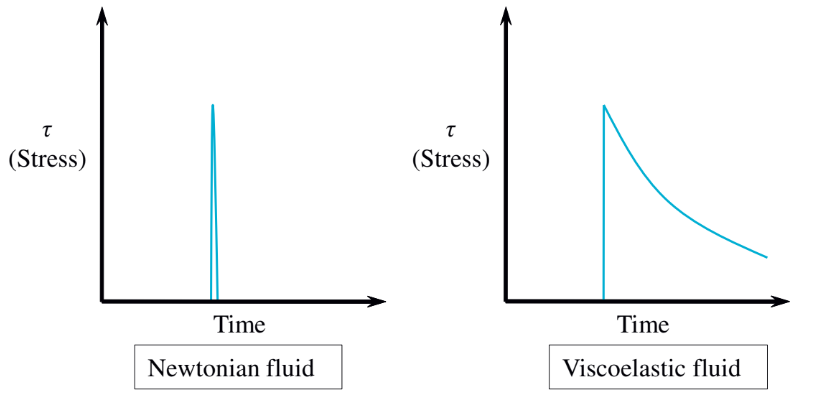
\includegraphics[scale=0.4]{Section_Files/S2-imagenes-Manuel/18.png}
\caption{Esquema de estrés de relajación entre un fluido Newtoneano (izquierda) y un fluido viscoelástico (derecha).}
\end{figure}
\end{frame}

\begin{frame}{Modelo de Maxwell para un fluido viscoelástico 01/02}
\justifying
Ejemplo de materiales biológicos que tienen un comportamiento viscoelástico: Piel, hueso, vasos sanguíneos.
\begin{figure}[H]
\centering
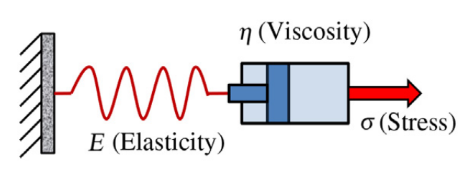
\includegraphics[scale=0.4]{Section_Files/S2-imagenes-Manuel/19.png}
\end{figure}
\end{frame}

\begin{frame}{Modelo de Maxwell para un fluido viscoelástico 02/02}
\begin{figure}
\centering
\subfloat{
\label{f:imagen1}
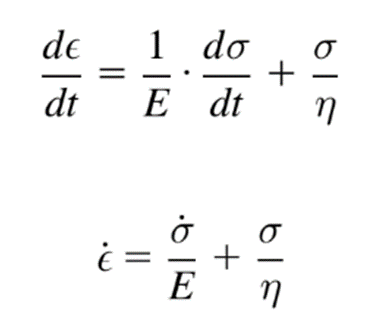
\includegraphics[height=0.2\textwidth]{Section_Files/S2-imagenes-Manuel/20.png}}
\subfloat{
\label{f:imagen2}

\includegraphics[height=0.2\textwidth]{Section_Files/S2-imagenes-Manuel/21.jpg}}
\caption{Where $ \epsilon $ is strain or deformation fraction. $E$ is elasticity module of material. $ \sigma $ is stree on material elements, $ \eta $ is viscosity and $ t $ is time.}
\label{f:casolagrangiano}
\end{figure}
\end{frame}

\begin{frame}{Viscoplástico}
\justifying
Un material viscoplástico necesita vencer un determinado esfuerzo propio de cada material para que pueda fluir, caso contrario el material se deformará.
\begin{figure}[H]
\centering
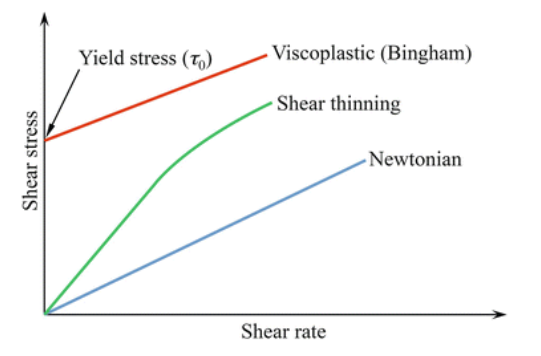
\includegraphics[scale=0.4]{Section_Files/S2-imagenes-Manuel/22.png}
\end{figure}
\end{frame}

\begin{frame}{Modelos para materiales viscoplástico}
\justifying
\begin{itemize}
\item Bingham
\item Herschel-Bulkley
\item Casson
\end{itemize}
\begin{figure}[H]
\centering
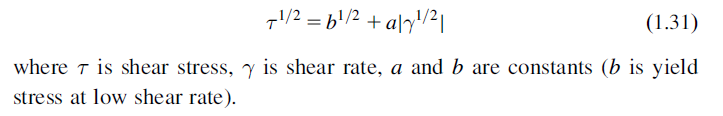
\includegraphics[scale=0.4]{Section_Files/S2-imagenes-Manuel/23.png}
\end{figure}
El módelo de Casson es aplicable a fluidos biológicos tales como la sangre.
\end{frame}